\section{Evaluation}
\label{sec:evaluation}

A reader who has followed the specification chapters this far has seen what \Flux claims to be.
This section checks the claim against the running network on one day, and against a small,
reproducible model of the monetary policy and of the not-yet-shipped \PNR mechanism. Three kinds
of number appear below, and each is labelled as it appears: a \emph{measured} number comes from a
live public endpoint queried on the date given; a \emph{modelled} number comes from executing a
pinned, deterministic script against consensus constants and is a projection, not an observation;
a \emph{derived} number is arithmetic performed on measured inputs (a percentage, a Gini
coefficient) and carries the same endpoint and date as the inputs it is computed from. Nothing
below is estimated from intuition, and where a quantity a reader might want is not obtainable at
all, that absence is stated rather than filled in.

\subsection{Methodology}
\label{sec:eval-methodology}

All measured figures in this section are read from \texttt{api.\allowbreak{}runonflux.\allowbreak{}io}, retrieved
2026-09-03, and are reproduced by \texttt{scripts/\allowbreak{}05-network-analysis.\allowbreak{}py}. Three endpoints are
used: \texttt{/\allowbreak{}daemon/\allowbreak{}getzelnodecount} and \texttt{/\allowbreak{}daemon/\allowbreak{}listzelnodes} for the fleet census,
payment rotation and operator-concentration figures (\S\ref{sec:eval-fleet}--\S\ref{sec:eval-concentration});
\texttt{/\allowbreak{}apps/\allowbreak{}globalappsspecifications} and \texttt{/\allowbreak{}apps/\allowbreak{}deploymentinformation} for the deployed
application set (\S\ref{sec:eval-apps}); and \texttt{/\allowbreak{}daemon/\allowbreak{}getblockchaininfo} for the shielded
value pools (\S\ref{sec:eval-shielded}). Chain tip at the time of the node-record query was height
2,917,115; the emission-model reference height, queried separately, was 2,912,015. The two differ
because they were captured at different points in the same collection run; both are stated
explicitly wherever they are used, and the difference (5,100 blocks, about 42.5 hours at 30 s
spacing) is immaterial to every figure below.

Modelled figures come from two independent, stdlib-only Python scripts, both executed
2026-09-03, both deterministic given the pinned constants they read, and both citable in full in
Appendix C: \texttt{flux-\allowbreak{}roadmap/\allowbreak{}supply/\allowbreak{}emission\_model.\allowbreak{}py} (with its generator
\texttt{\_gen\_dat.py}) for the supply and emission figures of \S\ref{sec:eval-supply}, and
\texttt{scripts/\allowbreak{}07-pnr-settlement.\allowbreak{}py} for the \PNR crossover and drip figures of
\S\ref{sec:eval-pnr-crossover}--\S\ref{sec:eval-drip}. The emission model reproduces already-shipped
consensus arithmetic (\PoN subsidy, halving history) and is stated in present tense; the \PNR
model projects a mechanism that is settled in design but not deployed, and is stated in future
tense throughout \S\ref{sec:eval-pnr-crossover}--\S\ref{sec:eval-drip}, consistent with its
\planned maturity.

Two absences are stated once here and not re-derived below. First, no public endpoint reports
realised utilisation, bandwidth, or latency of the deployed fleet — only the resources
\emph{requested} in application specifications are visible, and \S\ref{sec:eval-apps} reports
exactly that, with no estimate of what fraction is actually used. Second, the two identity proxies
available for operator concentration (\texttt{payment\_address}, \texttt{pubkey}) are lower bounds
on concentration by \emph{party}; no public endpoint links either to a real-world operator, so
every concentration figure in \S\ref{sec:eval-concentration} is stated as a lower bound, every time
it is used, not once and then dropped.

\subsection{The fleet}
\label{sec:eval-fleet}

This is a measured quantity, \shipped \srcmeasured{api.runonflux.io/\allowbreak{}daemon/\allowbreak{}getzelnodecount}{2026-09-03}.
The fleet has \textbf{6,489} nodes, all reported \texttt{stable}: 3,247 \FluxNode{}s enabled at
Cumulus, 1,615 at Nimbus, 1,627 at Stratus. \texttt{listzelnodes} returns 6,489 node records with
the same tier split; matched against per-tier collateral, the fleet locks \textbf{88,514,500 FLUX}
(Table~\ref{tab:eval-fleet}). Of the fleet, 2,322 nodes report an IPv4 address; none report IPv6 or
an onion address (0 of each), \shipped \srcmeasured{api.runonflux.io/\allowbreak{}daemon/\allowbreak{}getzelnodecount}{2026-09-03}.

\begin{table}[H]
\centering
\small
\begin{tabular}{lrrrr}
\toprule
tier & nodes & collateral each (FLUX) & tier collateral (FLUX) & share of voting power \\
\midrule
Cumulus & 3,247 & 1,000 & 3,247,000 & 3.67\% \\
Nimbus & 1,615 & 12,500 & 20,187,500 & 22.81\% \\
Stratus & 1,627 & 40,000 & 65,080,000 & 73.52\% \\
\midrule
total & 6,489 & --- & 88,514,500 & 100\% \\
\bottomrule
\end{tabular}
\caption{Fleet census by tier, measured 2026-09-03 at chain height 2,917,115. Voting weight is
collateral-weighted at one unit per 1,000 FLUX (88,514.5 weight units total).
\srcmeasured{api.runonflux.io/\allowbreak{}daemon/\allowbreak{}listzelnodes}{2026-09-03}.}
\label{tab:eval-fleet}
\end{table}

Node tenure, measured as blocks since \texttt{added\_height} across all 6,489 nodes
\shipped \srcmeasured{api.runonflux.io/\allowbreak{}daemon/\allowbreak{}listzelnodes}{2026-09-03}: median 193,620 blocks
(approximately 67 days at 30 s spacing), 10th percentile 12,909 blocks, 90th percentile 881,770
blocks, maximum 1,648,700 blocks. The fleet therefore contains both nodes confirmed within the
last collection window and nodes that predate \PoN activation by a wide margin; no further
resolution of the tenure distribution (a full histogram) is available from this endpoint.

\subsection{The payment rotation, measured}
\label{sec:eval-rotation}

Under \PoN, each tier's payment queue is ordered by ascending last-paid height, so a
deterministic rotation is a testable prediction: every node in a tier of $\ncount{t}$ nodes should
be paid at least once every $\ncount{t}$ blocks. Table~\ref{tab:eval-rotation} tests it directly
against the live payment queue \shipped \srcmeasured{api.runonflux.io/\allowbreak{}daemon/\allowbreak{}listzelnodes}{2026-09-03},
at tip height 2,917,115, by computing $\text{tip} - \text{last\_paid\_height}$ for every node.

\begin{table}[H]
\centering
\small
\begin{tabular}{lrrrrrr}
\toprule
tier & nodes & expected rotation (blocks) & max blocks since paid & median & 95th pct & rotation at 30 s \\
\midrule
Cumulus & 3,247 & 3,247 & 3,202 & 1,592 & 3,041 & 27.06 h \\
Nimbus & 1,615 & 1,615 & 1,597 & 800 & 1,517 & 13.46 h \\
Stratus & 1,627 & 1,627 & 1,631 & 807 & 1,545 & 13.56 h \\
\bottomrule
\end{tabular}
\caption{\PoN payment rotation, measured 2026-09-03 at chain tip 2,917,115.
\srcmeasured{api.runonflux.io/\allowbreak{}daemon/\allowbreak{}listzelnodes}{2026-09-03}.}
\label{tab:eval-rotation}
\end{table}

Cumulus and Nimbus stay strictly inside one rotation (max blocks-since-paid below the tier's node
count). Stratus exceeds its rotation length by 4 blocks (1,631 against 1,627), consistent with a
small number of nodes joining mid-cycle — at the measured median tenure of 67 days, roughly 1--2\%
of a tier's nodes join within any rotation-length window, and a join lengthens the cycle by exactly
one node without breaking the underlying period-$\ncount{t}$ structure. This measurement confirms
the deterministic one-node-per-tier-per-block rotation as a property of the deployed queue, not as
a model assumption: every node in a tier is paid within one rotation of that tier's node count,
equalising within 27.06 h (Cumulus), 13.46 h (Nimbus) and 13.56 h (Stratus). It is the empirical
basis for the fairness proposition of \S7 (that cumulative operator income within a tier is bounded
over one rotation) and is cited there directly.

\subsection{Operator concentration}
\label{sec:eval-concentration}

This is a derived quantity, computed from the fleet census
\shipped \srcmeasured{api.runonflux.io/\allowbreak{}daemon/\allowbreak{}listzelnodes}{2026-09-03}. Collateral-weighted
voting power (one unit per 1,000 FLUX) is aggregated by two identity proxies present in the public
record: \texttt{payment\_address}, where a node's rewards are sent, and \texttt{pubkey}, the node
key. Neither is proof of common ownership — one operator can use many addresses, and a shared
custodian can serve many operators — so \textbf{every figure in this subsection is a lower bound on
true concentration by party}, stated as such at each use, per the unresolved gap recorded as G12.

By \texttt{payment\_address}: 869 distinct identities control the full 88,514.5 weight units
(88,514,500 FLUX). A removal threshold of 25\% of total voting power is reached by the 4 largest
addresses (of 869, 0.46\%); 50\% by 19 addresses (2.19\%). The Gini coefficient of voting weight
across \texttt{payment\_address} is \textbf{0.8375}. By \texttt{pubkey}: 819 distinct identities
control the same total; 25\% is reached by the 3 largest keys (of 819, 0.37\%); 50\% by 16
(1.95\%). The Gini coefficient across \texttt{pubkey} is \textbf{0.8389}. Table~\ref{tab:eval-concentration}
gives both top-$N$ share curves in full.

\begin{table}[H]
\centering
\small
\begin{tabular}{rrr}
\toprule
top-$N$ identities & share, by \texttt{payment\_address} & share, by \texttt{pubkey} \\
\midrule
1 & 10.71\% & 10.71\% \\
5 & 28.07\% & 31.73\% \\
10 & 37.99\% & 41.56\% \\
20 & 51.19\% & 53.91\% \\
50 & 67.92\% & 69.31\% \\
100 & 78.88\% & 79.60\% \\
250 & 91.18\% & 91.84\% \\
\bottomrule
\end{tabular}
\caption{Cumulative share of collateral-weighted voting power held by the top-$N$ identities, by
two lower-bound proxies for operator identity. Measured 2026-09-03 at chain height 2,917,115.
\srcmeasured{api.runonflux.io/\allowbreak{}daemon/\allowbreak{}listzelnodes}{2026-09-03}.}
\label{tab:eval-concentration}
\end{table}

The largest single identity, by either proxy, holds 9,480.0 weight units (10.71\% of total voting
power) across 237 nodes; the most nodes held by any one identity is 479 (by \texttt{payment\_address})
or 480 (by \texttt{pubkey}). Restricting to Stratus alone, the same largest identity holds 14.57\%
of Stratus-only voting weight (9,480.0 of 65,080.0 weight units) and its node count there is exactly
237 — the largest identity's 237 nodes are entirely Stratus. Stratus-only concentration is somewhat
lower in Gini terms (0.7375 across 220 distinct \texttt{payment\_address} identities) than the
fleet-wide figures, but its top-1 share (14.57\%) is higher than the fleet-wide top-1 share (10.71\%)
because Stratus carries 73.52\% of total voting power in far fewer nodes.
Figure~\ref{fig:eval-concentration} plots the two fleet-wide cumulative-share curves of
Table~\ref{tab:eval-concentration}.

\begin{figure}[H]
\centering
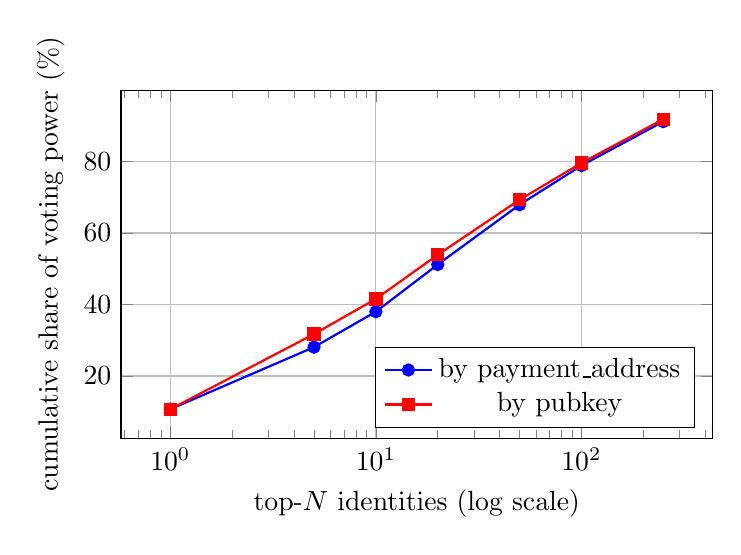
\begin{tikzpicture}
\begin{axis}[
  width=0.75\linewidth, height=6cm,
  xmode=log,
  xlabel={top-$N$ identities (log scale)},
  ylabel={cumulative share of voting power (\%)},
  legend pos=south east,
  grid=major,
]
\addplot[thick, blue, mark=*] coordinates {(1,10.71) (5,28.07) (10,37.99) (20,51.19) (50,67.92) (100,78.88) (250,91.18)};
\addplot[thick, red, mark=square*] coordinates {(1,10.71) (5,31.73) (10,41.56) (20,53.91) (50,69.31) (100,79.60) (250,91.84)};
\legend{by payment\_address, by pubkey}
\end{axis}
\end{tikzpicture}
\caption{Cumulative share of collateral-weighted voting power held by the top-$N$ operator
identities, by two lower-bound proxies. The curve is sampled at the seven $N$ values reported in
Table~\ref{tab:eval-concentration}, not at every $N$. Measured 2026-09-03 at chain height 2,917,115;
data underlying \texttt{paper/\allowbreak{}data/\allowbreak{}concentration\_payment\_address.\allowbreak{}dat} and
\texttt{paper/\allowbreak{}data/\allowbreak{}concentration\_pubkey.\allowbreak{}dat}. \srcmeasured{api.runonflux.io/\allowbreak{}daemon/\allowbreak{}listzelnodes}{2026-09-03}.}
\label{fig:eval-concentration}
\end{figure}

\subsection{Deployed applications}
\label{sec:eval-apps}

This is a measured quantity, \shipped \srcmeasured{api.runonflux.io/\allowbreak{}apps/\allowbreak{}globalappsspecifications}{2026-09-03}.
The endpoint returns \textbf{1,195} application specification records, comprising 1,371 components
(compose entries) and a total of \textbf{7,486} requested instances across all applications.
Instances per application: median 2, mean 6.26, maximum 100, minimum 0; 439 applications (36.7\%)
sit at the platform's 3-instance minimum. Table~\ref{tab:eval-appspec} gives the specification-version
distribution and Table~\ref{tab:eval-registry} the container-registry distribution.

\begin{table}[H]
\centering
\small
\begin{tabular}{lrr}
\toprule
spec version & applications & share \\
\midrule
v2 & 2 & 0.2\% \\
v3 & 27 & 2.3\% \\
v4 & 11 & 0.9\% \\
v5 & 3 & 0.3\% \\
v6 & 70 & 5.9\% \\
v7 & 209 & 17.5\% \\
v8 & 873 & 73.1\% \\
\bottomrule
\end{tabular}
\caption{Application specification version distribution, measured 2026-09-03.
\srcmeasured{api.runonflux.io/\allowbreak{}apps/\allowbreak{}globalappsspecifications}{2026-09-03}. \specv{9} does not yet
appear (\S10).}
\label{tab:eval-appspec}
\end{table}

\begin{table}[H]
\centering
\small
\begin{tabular}{lr}
\toprule
image registry & components \\
\midrule
\texttt{docker.io} (implicit) & 1,332 \\
\texttt{ghcr.io} & 31 \\
\texttt{quay.io} & 3 \\
\texttt{lscr.io} & 2 \\
\texttt{public.ecr.aws} & 1 \\
\texttt{ttl.sh} & 1 \\
\texttt{codeberg.org} & 1 \\
\bottomrule
\end{tabular}
\caption{Container registry distribution across 1,371 components, measured 2026-09-03.
\srcmeasured{api.runonflux.io/\allowbreak{}apps/\allowbreak{}globalappsspecifications}{2026-09-03}.}
\label{tab:eval-registry}
\end{table}

Summed committed resources across all 7,486 requested instances: 8,972.0 vCPU-equivalents,
17,544,229 MB of RAM (17,133.0 GiB), and 160,107 GB of disk. These are the resources declared in
application specifications and enforced at deployment time by the platform's own minimum/maximum
bounds (\texttt{minimum\allowbreak{}Instances}: 3, \texttt{maximum\allowbreak{}Instances}: 100,
\texttt{blocksLasting}: 22,000 blocks per default lifetime,
\srcmeasured{api.runonflux.io/\allowbreak{}apps/\allowbreak{}deploymentinformation}{2026-09-03}) — they are \emph{requested},
not realised. No public endpoint reports realised CPU, memory, disk or network utilisation of the
deployed fleet, and this section does not estimate it (G13); the committed-resource figures above
are the complete measurement available.

Feature usage across the 1,195 applications: \texttt{geolocation} 556 (46.5\%), \texttt{staticip}
50 (4.2\%), \texttt{nodes} (pinned placement) 11 (0.9\%), \texttt{enterprise} 223 (18.7\%),
\texttt{expire} 1,152 (96.4\%), \texttt{owner} 1,195 (100.0\%), \texttt{contacts} 699 (58.5\%),
\shipped \srcmeasured{api.runonflux.io/\allowbreak{}apps/\allowbreak{}globalappsspecifications}{2026-09-03}.

\subsection{Shielded value pools}
\label{sec:eval-shielded}

This is a measured quantity, \shipped \srcmeasured{api.runonflux.io/\allowbreak{}daemon/\allowbreak{}getblockchaininfo}{2026-09-03}.
At chain height 2,917,115, the \texttt{valuePools} field reports a Sapling pool of
\textbf{77,188.75921324 FLUX} and a Sprout pool of \textbf{19,291.17735041 FLUX}, both monitored,
for a combined shielded value of 96,479.93656365 FLUX. Consensus has rejected transparent-to-shielded
transfers since height 835,554 (\srccode{fluxd/\allowbreak{}src/\allowbreak{}main.cpp}{1398--1408}), so both pools have been
closed to new entrants since that height — 2,081,561 blocks before the measurement tip — and every
satoshi in them was shielded before the turnstile closed. Against the total issued supply of
429,466,823.9700 FLUX at height 2,912,015 (\S\ref{sec:eval-supply}), the shielded pools hold
\textbf{0.0225\%} of issued supply (derived). Note count and holder count of either pool are
\textbf{not obtainable} from this or any public endpoint and are not estimated here.

\subsection{Supply, modelled}
\label{sec:eval-supply}

This is a modelled quantity: it reproduces already-shipped \PoN consensus arithmetic
(\srccode{flux-roadmap/\allowbreak{}supply/\allowbreak{}emission\_model.py}{195--243}, itself a transcription of
\PoN's \texttt{Get\allowbreak{}Block\allowbreak{}Subsidy}) rather than a new mechanism, so it is stated \shipped and in
present tense, executed 2026-09-03 by \texttt{flux-\allowbreak{}roadmap/\allowbreak{}supply/\allowbreak{}emission\_model.\allowbreak{}py}
(\srcdoc{flux-roadmap/supply/emission\_model.py, run 2026-09-03}). Current issued supply at height
2,912,015 (mode \texttt{observed}, the model's default and the mode this paper uses for every
current-supply figure) is \textbf{429,466,823.9700 FLUX}. Mode \texttt{code} — a literal
transcription of \texttt{Get\allowbreak{}Block\allowbreak{}Subsidy()} — gives 429,466,973.9700 FLUX at the same height: a
persistent, height-independent offset of exactly \textbf{150.00000000 FLUX}, not the 0.06 FLUX the
model's own docstring claims, traced to a double-counted slow-start block in the \texttt{code}-mode
formula. This discrepancy, its derivation, and the reproduction instructions are given in full in
Appendix~C.

The \PoN subsidy started at \textbf{14 FLUX} per block at activation (height 2,020,000) and is
reduced by a factor of $9/10$ (with per-step integer truncation, so the reduction is not exactly
$0.9^r$) every $\redint = 1{,}051{,}200$ blocks — one year at 30 s spacing — for a maximum of
$\redmax = 20$ reductions (\srccode{flux-roadmap/\allowbreak{}supply/\allowbreak{}emission\_model.py}{149--150}). After the
20th reduction, the subsidy is frozen and does not decay further: at the onset of the tail (height
23,044,000, a 30-second-spacing extrapolation to approximately 2045-10-20; see
\S\ref{sec:eval-threats}), the block subsidy is fixed at 1.70207313 FLUX, and cumulative supply
grows without bound at a constant \textbf{1,789,219.274256 FLUX per year, forever}
(\srccode{flux-roadmap/\allowbreak{}supply/\allowbreak{}emission\_model.py}{514--546}). \textbf{There is no terminal supply.}
Supply at the end of PON year 20 (height 24,095,199, the last block before the flat-rate regime
begins) is 548,043,625.860464 FLUX; this is not a cap, only the point at which the annual emission
\emph{rate} becomes constant. The currently-issued 429,466,823.9700 FLUX is 78.36\% of that
year-20-onset level — a proxy for "how far along" the schedule is, stated explicitly as a proxy
rather than a fraction of a terminal supply, because no terminal supply exists to be a fraction of.
\texttt{MAX\_MONEY} (440,000,000 FLUX) is crossed by cumulative issuance at height 3,730,295
(approximately 2027-06-11); this is not a consensus failure, since \texttt{MAX\_MONEY} bounds a
single transaction's value, never the chain-wide supply accumulator.

\begin{figure}[H]
\centering
\begin{tikzpicture}
\begin{axis}[
  width=0.8\linewidth, height=6.5cm,
  xlabel={year}, ylabel={cumulative issued supply (FLUX)},
  grid=major,
  scaled y ticks=false, yticklabel style={/pgf/number format/fixed, /pgf/number format/1000 sep=\,},
]
\addplot[thick, blue] table[x index=0, y index=2] {../data/emission.dat};
\end{axis}
\end{tikzpicture}
\caption{Cumulative issued FLUX supply, 2026--2060, mode \texttt{observed}. The curve is a
straight line in the flat tail from approximately 2045 onward (1,789,219.274256 FLUX/yr) and never
asymptotes. \srcdoc{flux-roadmap/supply/emission\_model.py, run 2026-09-03}; data in
\texttt{paper/\allowbreak{}data/\allowbreak{}emission.\allowbreak{}dat} (columns: year, height, cumulative\_supply, annual\_emission,
pow\_emission, pon\_emission).}
\label{fig:eval-supply}
\end{figure}

\begin{figure}[H]
\centering
\begin{tikzpicture}
\begin{axis}[
  width=0.8\linewidth, height=6.5cm,
  xlabel={year}, ylabel={modelled annual operator income per node (FLUX/yr)},
  legend pos=north east,
  grid=major,
]
\addplot[thick, blue] table[x index=0, y index=1] {../data/tier_income.dat};
\addplot[thick, red] table[x index=0, y index=2] {../data/tier_income.dat};
\addplot[thick, black] table[x index=0, y index=3] {../data/tier_income.dat};
\legend{Cumulus, Nimbus, Stratus}
\end{axis}
\end{tikzpicture}
\caption{Modelled per-node \PoN issuance income by tier, 2026--2060, at a fixed fleet
(3,246 / 1,615 / 1,627 nodes, held constant; fleet growth and churn are not modelled). Per-node
income scales with tier subsidy share and inversely with tier node count, not with collateral
(\Cref{prop:pnr:across}). \srcdoc{flux-roadmap/supply/emission\_model.py, run 2026-09-03}; data in
\texttt{paper/\allowbreak{}data/\allowbreak{}tier\_income.\allowbreak{}dat} (columns: year, cumulus\_per\_node, nimbus\_per\_node,
stratus\_per\_node, cumulus\_total, nimbus\_total, stratus\_total, total).}
\label{fig:eval-tier-income}
\end{figure}

\subsection{The PNR crossover, modelled, in both denominations}
\label{sec:eval-pnr-crossover}

\PNR does not exist in deployed code. As of the measurement tip (height 2,917,115), the chain is
549,515 blocks short of the planned activation height $\hpa = 3{,}466{,}630$ (approximately
2027-03-12 at 30 s spacing). Everything in this subsection is therefore a \planned projection —
\srcintent{design intake} for the settled design (an 80\%/20\% Foundation/operator
split at activation, ramping by 5 percentage points at each \PoN reduction to a cap of 50\%), and
\srcdoc{scripts/07-pnr-settlement.py, run 2026-09-03} for every number computed from it — and is
stated in future tense throughout. It is stated in both FLUX terms (primary, because FLUX is what
consensus governs) and real terms (secondary, with a price multiple treated as an exogenous axis,
not a forecast); the two must never be used to defend one another. This paper makes no price
prediction anywhere in what follows.

The crossover model uses a fleet fixed at 3,246 / 1,615 / 1,627 nodes (6,488 total) — one Cumulus
node fewer than \S\ref{sec:eval-fleet}'s measured 3,247 / 1,615 / 1,627 (6,489), a one-node
difference between census windows that changes nothing at the precision reported below. It also
uses a \emph{planned} subsidy path distinct from the as-coded schedule of Figure~\ref{fig:eval-supply}:
from $\hpa$, the \PoN subsidy is additionally halved on top of the ordinary $9/10$ reduction
schedule (14 $\to$ 12.6 $\to$ 6.3 FLUX at $\hpa$, then 5.67, 5.103, \ldots), a change that
\texttt{paper/\allowbreak{}data/\allowbreak{}emission.\allowbreak{}dat} does not contain.

\textbf{At activation}, with $\nodeshare(\hpa) = 0.20$ and subsidy 6.3 FLUX, modelled operator
issuance (excluding the dev-fund remainder) would be 6,386,040 FLUX/yr. Under the team's activation-scale
revenue assumption $V_0 = 1{,}431{,}600$ FLUX/yr (1,193 applications $\times$ 100 FLUX/month
$\times$ 12 — a modelling assumption, not a measured receipt total; O17 in \S7), \PNR income would
be $0.20 \times V_0 = 286{,}320$ FLUX/yr. \textbf{\PNR would be 4.29\% of total operator income at
activation} (\PNR as a share of \PoN issuance plus \PNR combined: $286{,}320 / 6{,}672{,}360$).
"Parity" — the point at which \PNR income would equal \PoN issuance income — would require annual
application revenue of \textbf{31,930,200 FLUX/yr}, 22.3$\times$ $V_0$, at activation.

\begin{table}[H]
\centering
\small
\begin{tabular}{lllrrrr}
\toprule
stage start ($\hgt$) & date & subsidy (FLUX) & $\nodeshare$ & operator issuance (FLUX/yr) & parity revenue (FLUX/yr) & growth from $V_0$ \\
\midrule
3,466,630 & 2027-03-12 & 6.3000 & 0.20 & 6,386,040 & 31,930,200 & --- \\
4,122,400 & 2027-10-25 & 5.6700 & 0.25 & 5,747,436 & 22,989,744 & 16.1$\times$ \\
5,173,600 & 2028-10-24 & 5.1030 & 0.30 & 5,172,692 & 17,242,308 & 12.0$\times$ \\
6,224,800 & 2029-10-24 & 4.5927 & 0.35 & 4,655,423 & 13,301,209 & 9.3$\times$ \\
7,276,000 & 2030-10-24 & 4.1334 & 0.40 & 4,189,881 & 10,474,702 & 7.3$\times$ \\
8,327,200 & 2031-10-24 & 3.7201 & 0.45 & 3,770,893 & 8,379,762 & 5.9$\times$ \\
9,378,400 & 2032-10-23 & 3.3481 & 0.50 (cap) & 3,393,803 & 6,787,607 & 4.7$\times$ \\
12,532,000 & 2035-10-23 & 2.4407 & 0.50 & 2,474,083 & 4,948,165 & 3.5$\times$ \\
17,788,000 & 2040-10-21 & 1.4412 & 0.50 & 1,460,921 & 2,921,842 & 2.0$\times$ \\
23,044,000 & 2045-10-20 & 0.8510 & 0.50 & 862,659 & 1,725,319 & 1.2$\times$ (perpetual tail) \\
\bottomrule
\end{tabular}
\caption{Planned \PNR schedule in FLUX terms (primary), modelled 2026-09-03. Dates are 30-second-spacing
extrapolations (\S\ref{sec:eval-threats}). \srcintent{design intake};
\srcdoc{scripts/07-pnr-settlement.py, run 2026-09-03}.}
\label{tab:eval-pnr-flux}
\end{table}

The two levers (falling subsidy, rising $\nodeshare$) would together bring the parity requirement
down from 31.9 M to 6.8 M FLUX/yr over 5.6 years and to 1.7 M FLUX/yr on the perpetual tail. Whether
demand ever reaches that requirement is a separate question, answered only under explicit,
stated assumptions about revenue growth $g$ — never as a forecast. Table~\ref{tab:eval-pnr-growth}
gives the modelled crossover year under six such assumptions ($g \in \{0\%, 10\%, 25\%, 50\%,
100\%, 200\%\}$ per year, constant from $V_0$); these are scenario axes chosen to span a wide
range, not predictions of which growth rate, if any, will occur.

\begin{table}[H]
\centering
\small
\begin{tabular}{lccc}
\toprule
$g$ (per year) & crossover & revenue at crossover (FLUX/yr) & $\nodeshare$ at crossover \\
\midrule
0\% & never & --- & --- \\
10\% & 2038-10 & 4.33 M & 0.50 \\
25\% & 2033-10 & 6.28 M & 0.50 \\
50\% & 2031-10 & 9.33 M & 0.45 \\
100\% & 2030-10 & 17.6 M & 0.40 \\
200\% & 2029-10 & 25.6 M & 0.35 \\
\bottomrule
\end{tabular}
\caption{Modelled crossover year under constant annual revenue growth from $V_0$.
\srcdoc{scripts/07-pnr-settlement.py, run 2026-09-03}; data in \texttt{paper/\allowbreak{}data/\allowbreak{}pnr\_crossover.\allowbreak{}dat}
(columns \texttt{pnr\_g000}\ldots\texttt{pnr\_g200}).}
\label{tab:eval-pnr-growth}
\end{table}

\textbf{Under flat demand ($g = 0\%$), there is no crossover, ever.} The perpetual tail issuance
(862,659 FLUX/yr) exceeds $\nodesharecap \cdot V_0 = 715{,}800$ FLUX/yr, so even at the ramp's cap
of 50\%, \PNR income at flat $V_0$ would never reach \PoN issuance income; the parity requirement
falls over time only because the subsidy keeps falling, and reaching it is a statement about demand
growth, never about the subsidy schedule alone. Sustained growth required to reach parity by a
given year: 134\%/yr by 2029, 73\%/yr by 2030, 47\%/yr by 2031, 32\%/yr by 2032, 25\%/yr by 2033,
16\%/yr by 2035. As scheduled, \PNR would begin as a supplement to operator income; whether it ever
becomes the dominant component is a statement about demand that this paper does not make.

\begin{table}[H]
\centering
\small
\begin{tabular}{lccccc}
\toprule
$g$ \textbackslash\ $m$ & 0.5 & 1 & 2 & 5 & 10 \\
\midrule
0\% & 14.6 & never & never & never & never \\
10\% & 7.6 & 11.6 & 14.6 & 19.6 & 26.1 \\
25\% & 5.6 & 6.6 & 9.6 & 11.6 & 13.6 \\
50\% & 3.6 & 4.6 & 5.6 & 7.6 & 9.6 \\
100\% & 2.6 & 3.6 & 4.6 & 5.6 & 5.6 \\
\bottomrule
\end{tabular}
\caption{Modelled years to \PNR parity, real terms (secondary), under real demand growth $g$
(rows) and an exogenous FLUX price multiple $m$ (columns; $m > 1$ denotes FLUX-price appreciation
against the rebased price table, $m$ is a modelling axis, not a forecast). Under rebasing, price
appreciation \emph{delays} FLUX-terms parity even as real operator income rises — the two
statements are made in different denominations and this paper does not use one to defend the other.
\srcdoc{scripts/07-pnr-settlement.py, run 2026-09-03}; data in
\texttt{paper/\allowbreak{}data/\allowbreak{}pnr\_crossover\_real.\allowbreak{}dat}.}
\label{tab:eval-pnr-real}
\end{table}

\subsection{The drip trade-off}
\label{sec:eval-drip}

This subsection is also \planned and modelled, \srcdoc{scripts/07-pnr-settlement.py, run 2026-09-03},
and supports the settled value \drip = 86,400 blocks (30 days at 30 s spacing) of \S7. The
drip constant $\drip$ trades intra-rotation income spread and activation lag against timing-attack
resistance and pool size. Table~\ref{tab:eval-drip} gives the trade-off at the five candidate values
computed in \texttt{paper/\allowbreak{}data/\allowbreak{}pnr\_drip.\allowbreak{}dat}, against the longest rotation in the fleet (Cumulus,
3,246 nodes in the settlement model).

\begin{table}[H]
\centering
\small
\begin{tabular}{rrrrrr}
\toprule
$\drip$ (blocks) & half-life (days) & decay-side spread$^{\downarrow}$ & one-Stratus recapture & ramp to 95\% (days) & pool at parity (FLUX) \\
\midrule
3,246 & 0.78 & 171.79\% & 0.0205\% & 3.4 & 49,000 \\
10,000 & 2.41 & 38.34\% & 0.0067\% & 10.4 & 152,000 \\
32,460 & 7.81 & 10.51\% & 0.0021\% & 33.7 & 493,000 \\
64,920 & 15.62 & 5.13\% & 0.0010\% & 67.6 & 986,000 \\
\textbf{86,400} & \textbf{20.79} & \textbf{3.83\%} & \textbf{0.00077\%} & \textbf{90} & \textbf{1,310,000} \\
\bottomrule
\end{tabular}
\caption{Modelled drip trade-off at the measured Cumulus rotation length. Decay-side spread is the
first-versus-last-payee income ratio within one Cumulus rotation under zero inflow; recapture is
the fraction of its own \PNR payment a single Stratus node could recover by timing that payment,
against the $10^{-4}$ threshold of requirement H5. Ramp is the time to reach 95\% of steady-state
drip from a zero pool at activation. Pool at parity is the modelled steady-state pool at
parity-scale revenue and $\nodeshare = 0.50$. \srcdoc{scripts/07-pnr-settlement.py, run 2026-09-03};
data in \texttt{paper/\allowbreak{}data/\allowbreak{}pnr\_drip.\allowbreak{}dat}.}
\label{tab:eval-drip}
\end{table}

The settled $\drip = 86{,}400$ would leave one Stratus operator able to recover at most
0.00077\% of its own operator share by timing a payment to its own payout — three orders of
magnitude below the $10^{-4}$ threshold this paper sets for a negligible timing attack — at the
cost of a 20.79-day half-life and a roughly 90-day ramp to steady state after activation, since the
pool is not seeded (settled, O11 in \S7). At parity-scale revenue, the modelled steady-state
pool would hold approximately 1.31 M FLUX; this paper states plainly, per \S7's own framing, that
this balance would be a delay line with a 30-day time constant, not a treasury.

\subsection{Threats to validity}
\label{sec:eval-threats}

The measurements of \S\ref{sec:eval-fleet}--\S\ref{sec:eval-shielded} are a \textbf{single-day
snapshot}, taken 2026-09-03; fleet size, rotation state, application counts and concentration all
change continuously, and no time series is reported here beyond the node-tenure distribution.
Operator-concentration figures (\S\ref{sec:eval-concentration}) are, by construction, \textbf{lower
bounds}: \texttt{payment\_address} and \texttt{pubkey} are the only public identity proxies, and
true concentration by economic party is not obtainable from any public endpoint (G12); this paper
does not claim to know it. Application resource figures (\S\ref{sec:eval-apps}) are
\textbf{requested, not realised}: no public endpoint reports actual CPU, memory, disk, bandwidth or
latency utilisation of the deployed fleet, and none of the committed-resource figures should be
read as a utilisation claim (G13). The supply and \PNR projections of
\S\ref{sec:eval-supply}--\S\ref{sec:eval-drip} assume a \textbf{constant 30-second block spacing}
for every height and date beyond the current tip; the emission model's own validation states this
assumption is accurate to within approximately 0.8 days after 796,820 blocks, and is explicitly
unquantified over the multi-decade horizons (the year-20 tail onset, approximately 2045) that this
section cites — real \PoN spacing may drift, and every calendar date attached to a future height
carries that uncertainty. Finally, the \PNR crossover figures rest on a single, team-supplied
activation-scale revenue assumption ($V_0 = 1{,}431{,}600$ FLUX/yr; O17 in \S7) rather than a
measured receipt total, and the growth rates $g$ and price multiples $m$ used to project beyond it
are modelling axes chosen to span a range, not forecasts of what will occur — this paper makes no
claim about which, if any, will be realised.

%% Drain this section's float queue before the next begins.
\FloatBarrier
